\chapter{Diagrams}
\ChapterLabel{Diagrams}

\section{Browse and Access Research Projects}

This diagram explains the search interaction supporting
\RequirementRef{REQ-Q-006}
and \RequirementRef{REQ-Q-009}.

\begin{figure}[h!]
\centering
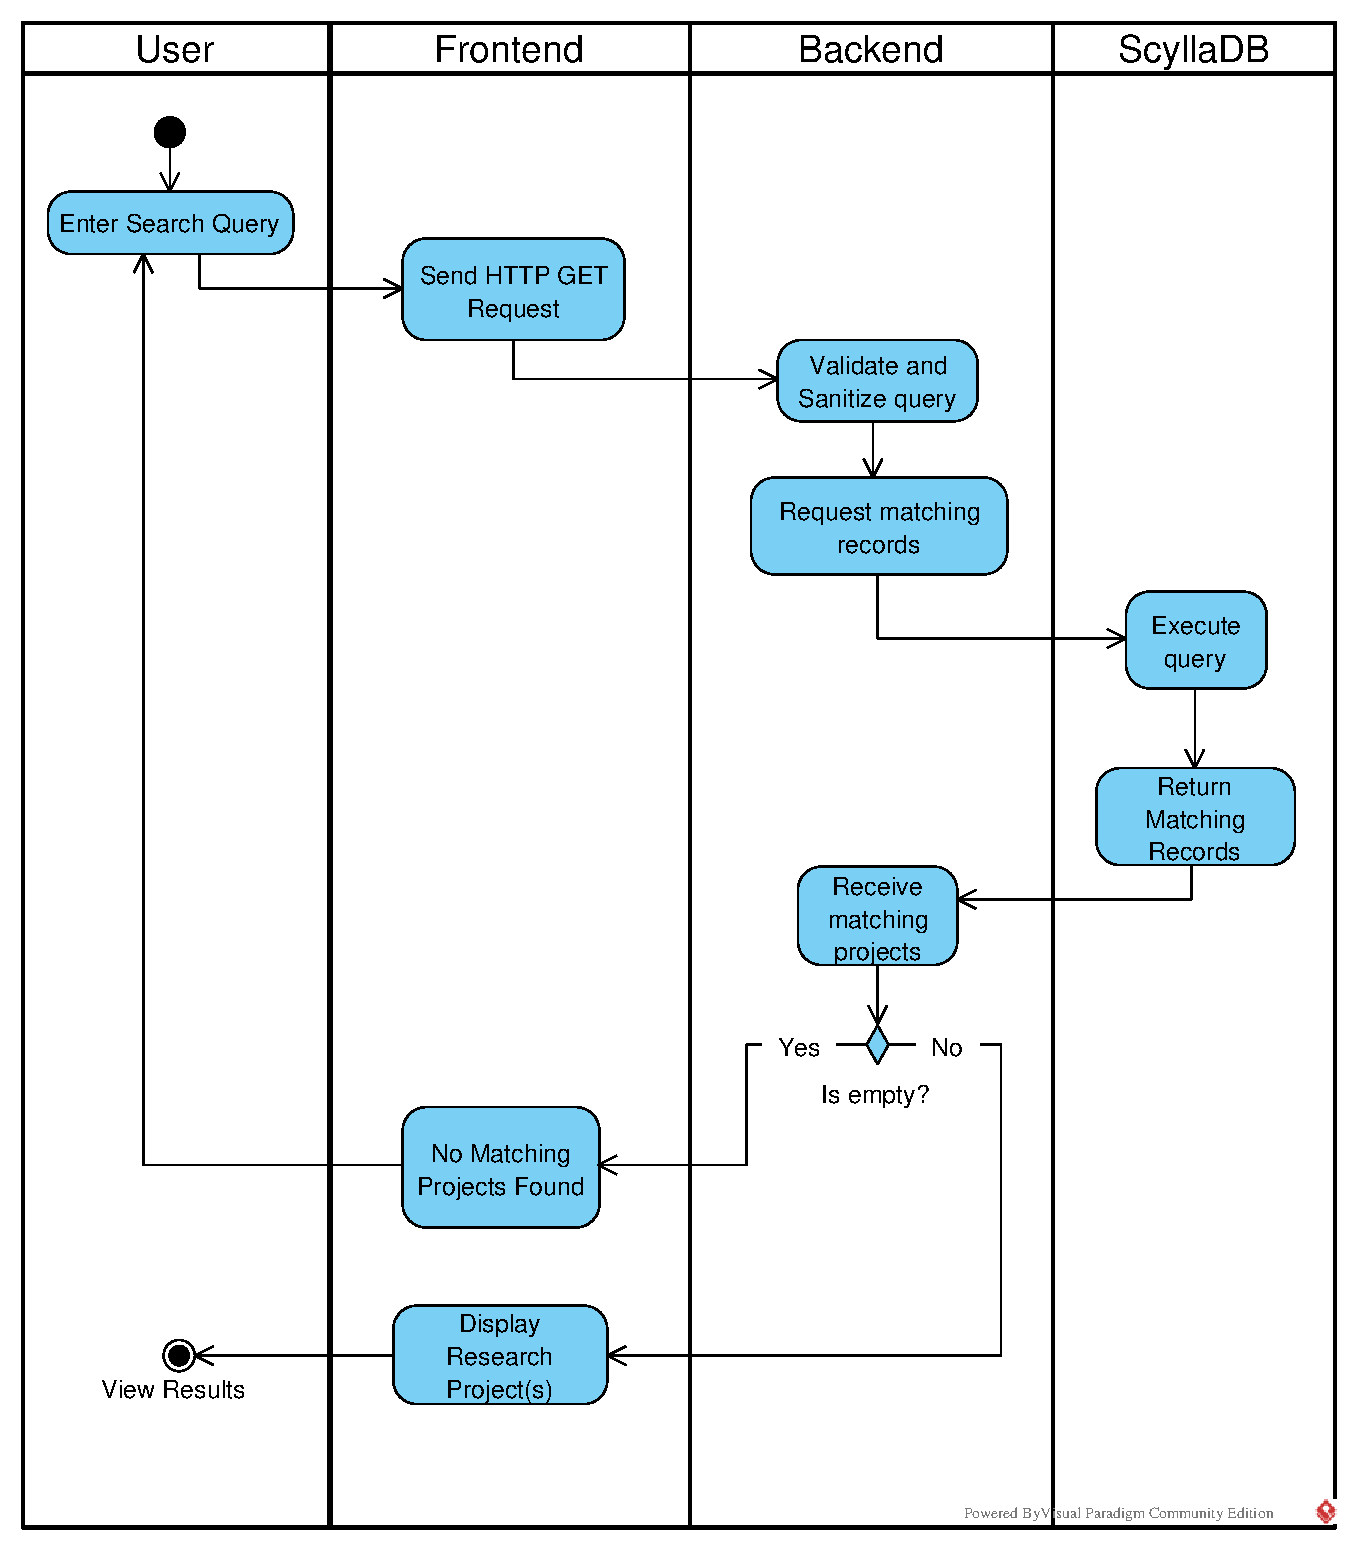
\includegraphics[width=0.65\textwidth]{diagrams/dsnUseCases/Swimlane.eps}
\caption{Search Function Sequence Diagram}
\label{Figure:SearchSequenceDiagram}
\end{figure}

\clearpage


\section{Manage Collaboration and Access}

The permission-management activity supports
\RequirementRef{REQ-S-001},
\RequirementRef{REQ-S-002}, and
\RequirementRef{REQ-F-005}.

\begin{figure}[h!]
\centering
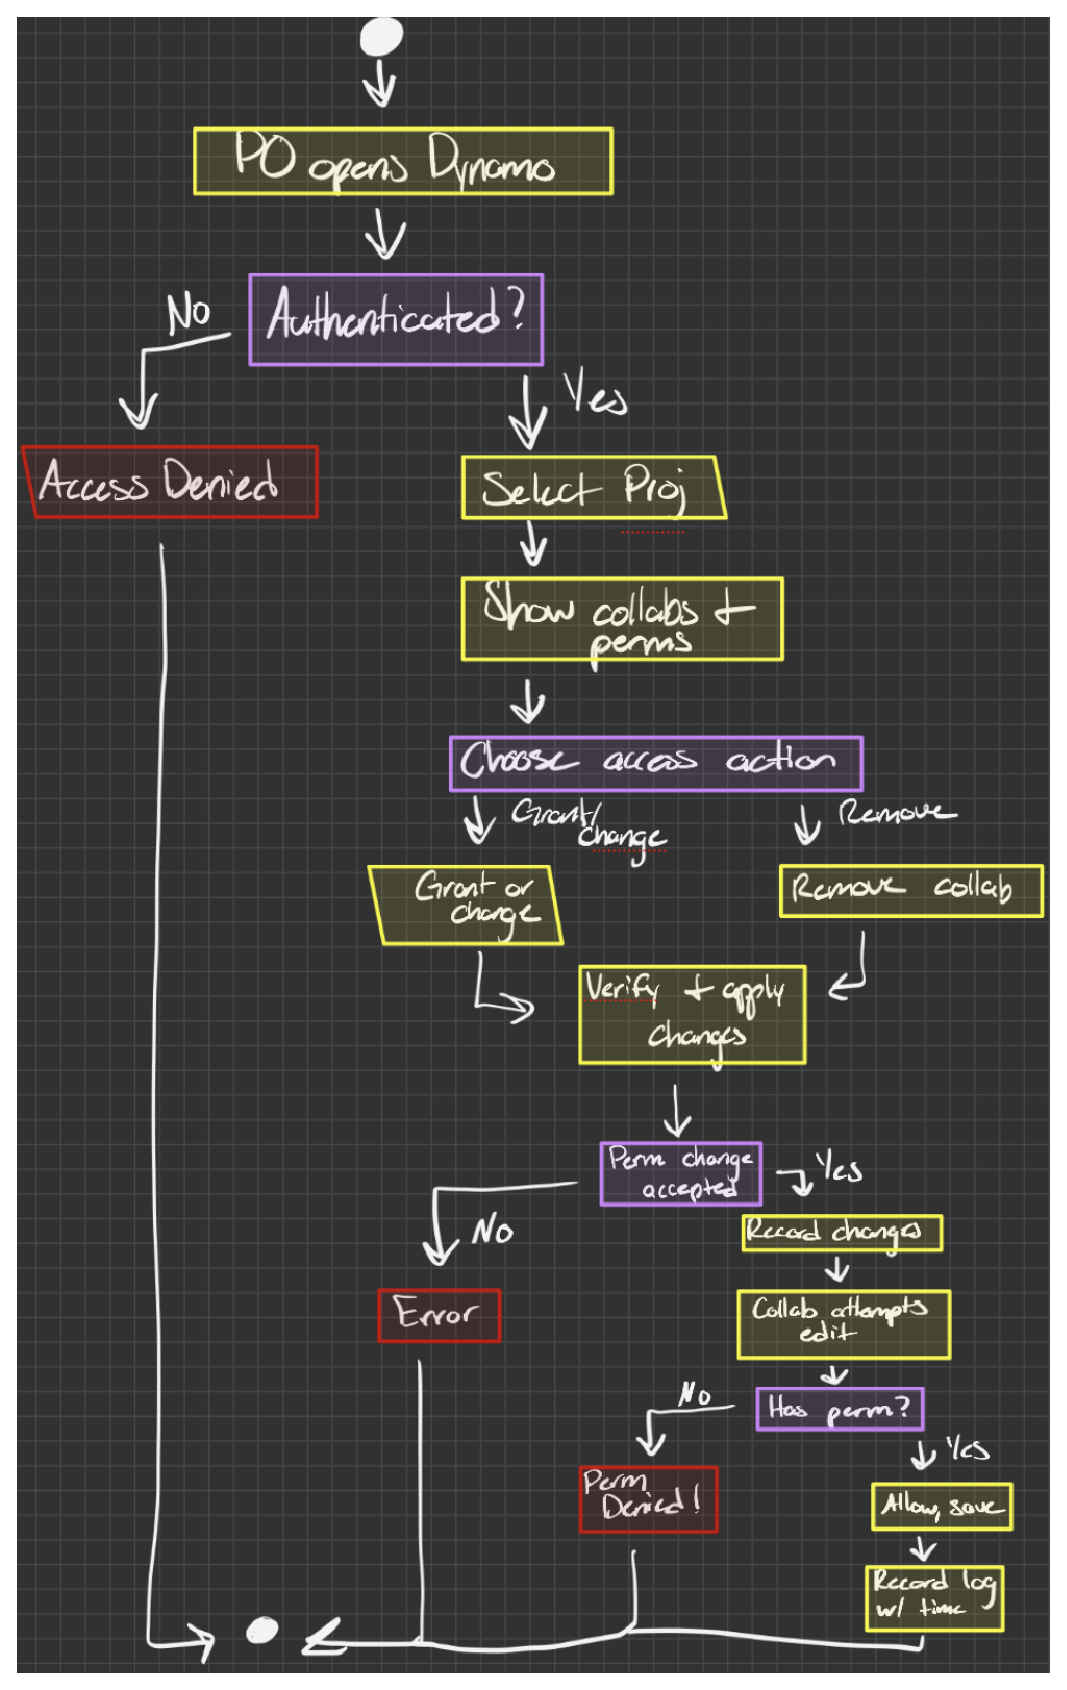
\includegraphics[width=0.5\textwidth]{eps/dsnUseCases/ManageCollaborationAndAccessActivityDiagram.eps}
\caption{Manage Collaboration And Access Use Case Diagram. \label{Figure:ManageCollaborationAndAccessUseCaseDiagram}}
\end{figure}
\index{use case diagram}

\clearpage

\section{Register a Published Paper Using a DOI}

Supports
\RequirementRef{REQ-F-003},
\RequirementRef{REQ-F-004},
\RequirementRef{REQ-F-005}, and
\RequirementRef{REQ-D-007}.

\begin{figure}[h!]
\centering
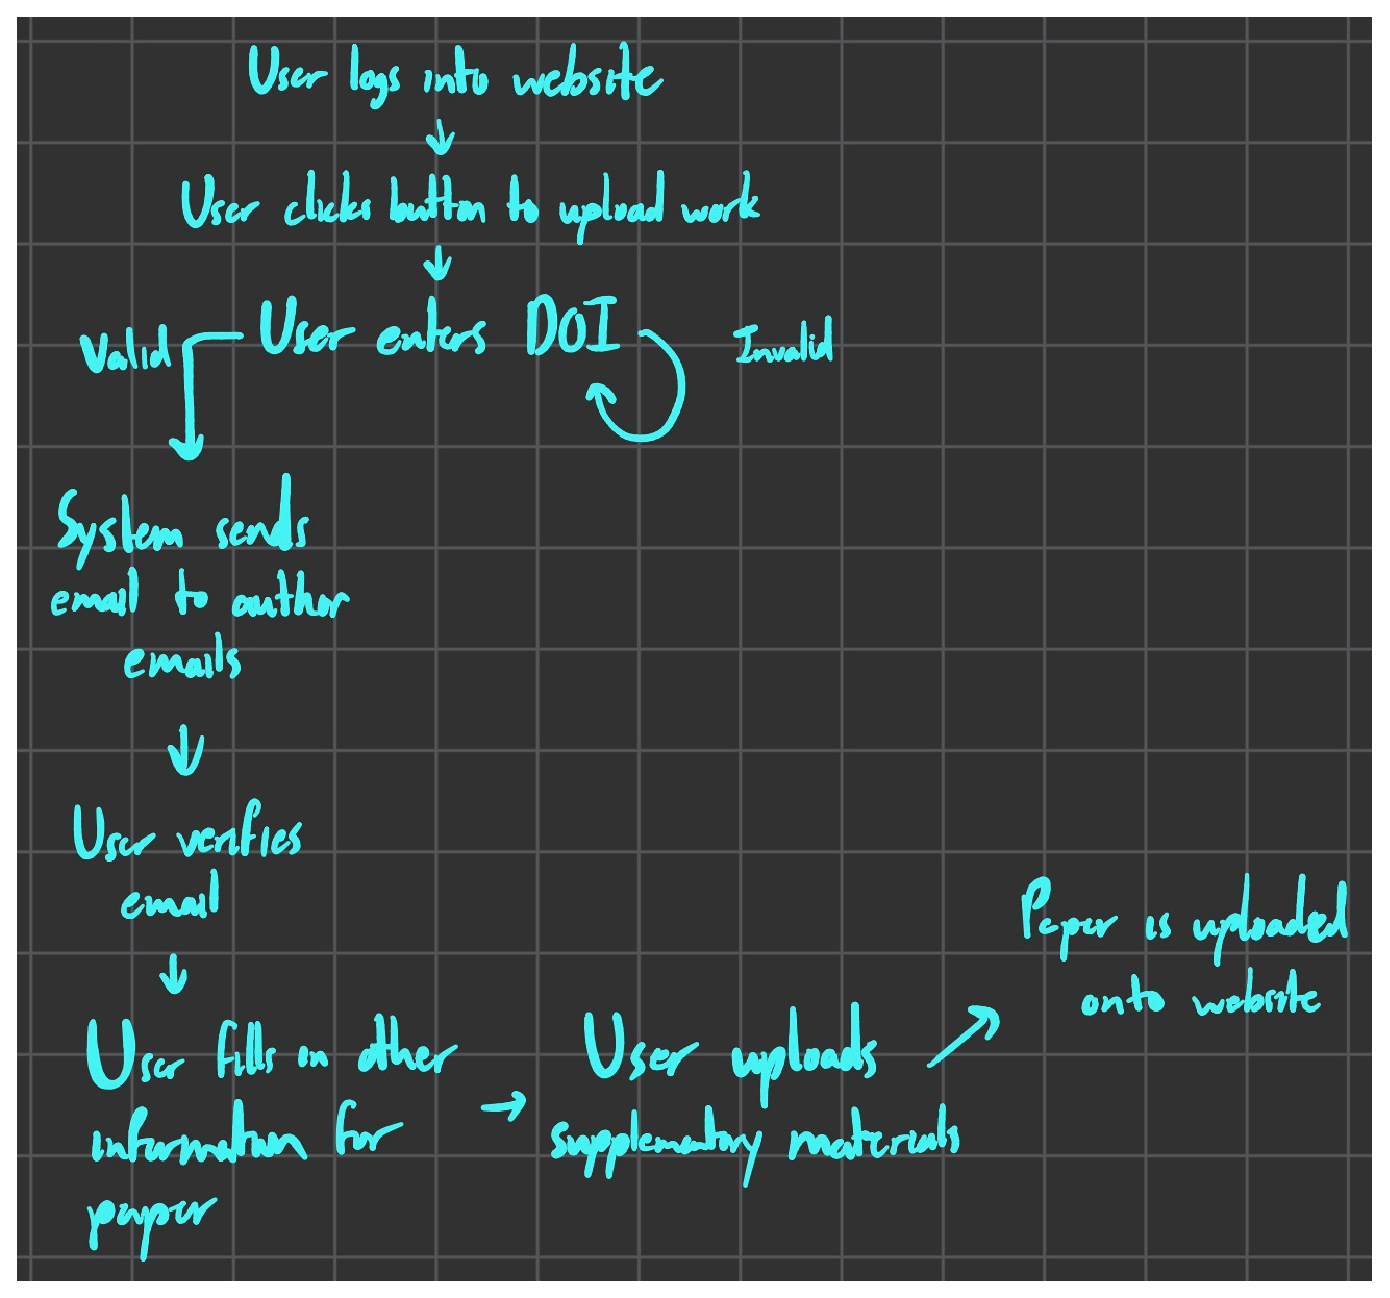
\includegraphics[width=0.5\textwidth]{eps/dsnUseCases/UploadDocumentActivityDiagram.eps}
\caption{Register a Published Paper Using a DOI Use Case Diagram.\label{Figure:DOIUploadUseCaseDiagram}}
\end{figure}
\index{use case diagram}

\clearpage

\section{Manage Research Artifacts}

This workflow supports
\RequirementRef{REQ-D-001},
\RequirementRef{REQ-Q-001},
\RequirementRef{REQ-Q-002},
\RequirementRef{REQ-Q-003},
\RequirementRef{REQ-S-001},
\RequirementRef{REQ-I-001}, and
\RequirementRef{REQ-D-008}.

The following diagrams describe the researcher-facing
workflow and proposed system components.

\subsection{Use Case Diagram}

The use case diagram shows the researcher's upload and
modification interactions, including authorization
and provenance recording.

\begin{figure}[htbp]
\centering
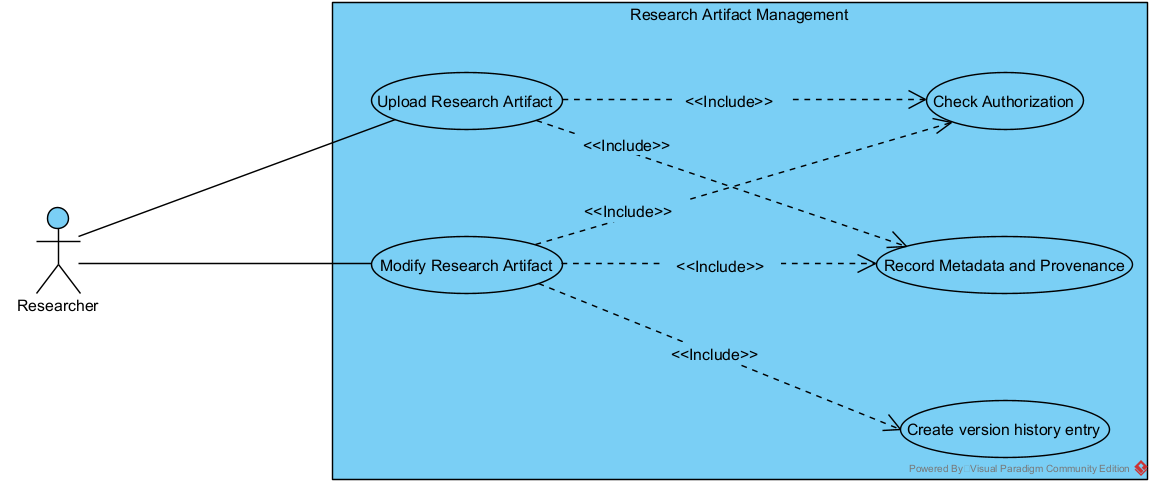
\includegraphics[width=1.05\textwidth,height=0.72\textheight,keepaspectratio]{png/UC-005 Use Case Diagram.png}
\caption{UC-005 Manage Research Artifacts Use Case Diagram}
\label{fig:uc005-usecase}
\end{figure}

\clearpage

\subsection{Activity Diagram}

The activity diagram shows the authorization decision,
artifact validation, success and failure paths,
and version-history creation.

\begin{figure}[htbp]
\centering
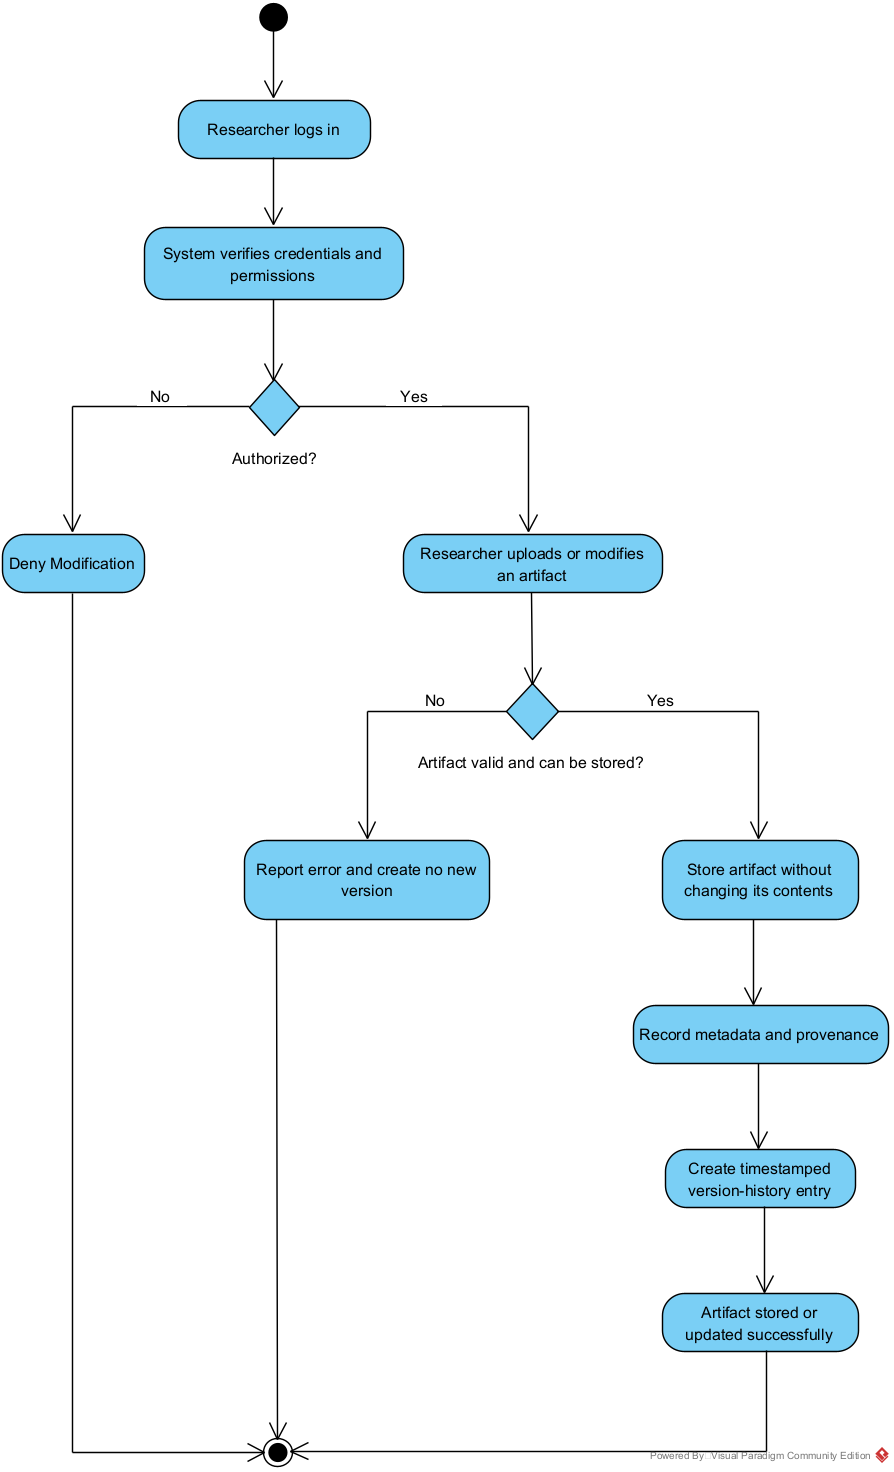
\includegraphics[width=0.8\textwidth,height=0.68\textheight,keepaspectratio]{png/UC-005ActivityDiagram.png}
\caption{UC-005 Manage Research Artifacts Activity Diagram}
\label{fig:uc005-activity}
\end{figure}

\clearpage

\subsection{Component Diagram}

The component diagram shows the React frontend,
Node.js and Express backend, authentication and
authorization, version management, ScyllaDB,
and file storage.

\begin{figure}[htbp]
\centering
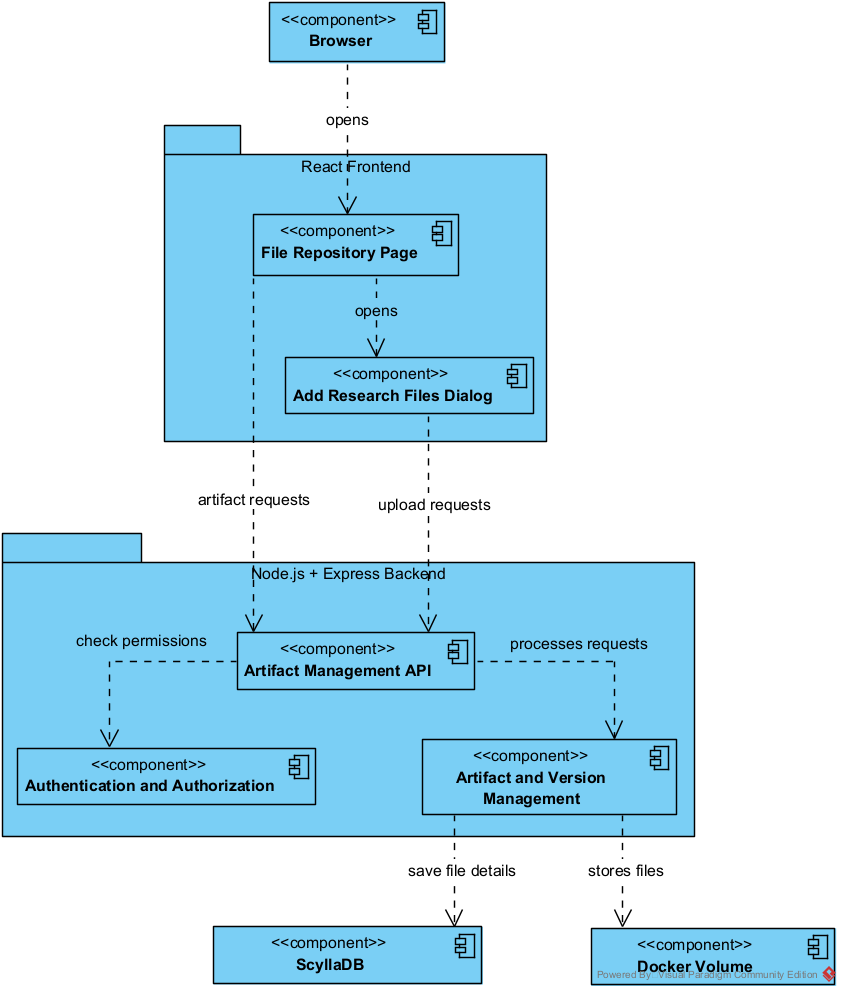
\includegraphics[width=0.95\textwidth,height=0.70\textheight,keepaspectratio]{png/UC-005 Component Diagram.png}
\caption{UC-005 Manage Research Artifacts Component Diagram}
\label{fig:uc005-component}
\end{figure}
\newpage
\subsection{MVC Diagram}

This diagram shows the interaction between the View, Controller, and Model of the platform
\begin{figure}[h!]
\centering
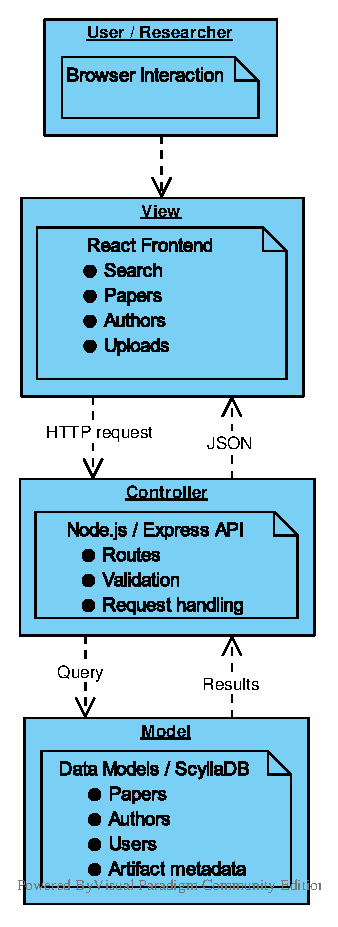
\includegraphics[width=0.35\textwidth]{eps/MVC_Diagram.eps}
\caption{MVC diagram of the Dynamo platform. \label{Figure:MVCDiagram}}
\end{figure}
\index{MVC Diagram}

\clearpage
